\section{Findings Ledger Index}
\label{app:ledger}

The paper cites findings by identifier. Each identifier is an entry in \repo{FINDINGS.md}, which records
for every result its exact numbers, the models involved, its evidence class, its status (exploratory,
confirmed, held-out confirmed, negative), a reproduction pointer (configuration, command and artifact
path) and an interestingness score from 1 to 5. The ledger is curated from the research log on the
\texttt{dev} branch and includes negative results on equal terms. Section letters: SH shared vs.\ unique
representations; CA causal agreement; DE depth; PM per-model character; MP method positives; MN method
negatives; BM benchmark trust. Table~\ref{tab:ledger} indexes the entries cited here.

\begin{center}
\scriptsize
\setlength{\tabcolsep}{3pt}
\begin{longtable}{@{}l>{\raggedright}p{8.6cm}>{\raggedright}p{2.6cm}c@{}}
\caption{Ledger entries cited in this paper (score = interestingness, 1--5).}\label{tab:ledger}\\
\toprule
ID & Claim (abridged) & Evidence / status & Score \\
\midrule
\endfirsthead
\toprule
ID & Claim (abridged) & Evidence / status & Score \\
\midrule
\endhead
\bottomrule
\endfoot
SH-01 & Peak CKA 0.38--0.47 above shuffled-series nulls (0.02--0.16) across five architectures, including Timer via the zero-code adapter & geometric; exploratory & 5 \\
SH-05 & CKA and clustering AMI rank model pairs differently on three panels & geometric vs.\ descriptive; replicated & 5 \\
SH-10 & Joint crosscoder loses to independent post-hoc-matched SAEs (0.2787 vs.\ 0.3204, $p=0.002$), pre-registered & correlational; negative & 5 \\
SH-14 & Concept transfer on shared inputs vs.\ stratum-matched null: 56.3\% forward, 46.1\% reciprocal; uniform null gave false 30/30 & correlational; exploratory & 5 \\
SH-16 & No atlas concept spans all four models; convergent is the modal sharing class & descriptive over causal parts; exploratory & 5 \\
SH-18 & Registered concept-transfer claims confirmed on private data: 19/20, 20/20 frozen, 20/20 on v2 & held-out confirmed & 5 \\
SH-19 & Unit-level correspondence fails rotation controls (0.148 $\to$ 0.331); participation ratio as low as 1.54 & geometric; negative & 5 \\
SH-20 & 11 of 13 targets non-modular once a minimum cluster size is enforced & descriptive; confirmed & 4 \\
CA-01 & Perturbation-fingerprint agreement is pair-specific; TimesFM/Chronos-2 replicates on private data & causal within-model; held-out & 4 \\
CA-03 & Seasonality circuit: 1 head (TimesFM) vs.\ 5 non-additive heads (Chronos-T5-Base) & causal within-model; exploratory & 4 \\
CA-04 & Attention mass at seasonal lags uncorrelated with causal importance ($\rho=0.026$, $-0.118$) & causal vs.\ descriptive; exploratory & 4 \\
CA-06 & On shared inputs with matched floors, most apparent cross-model disagreement disappears (18/19 $\to$ 12/89) & causal on shared inputs; exploratory, 2 corpora & 5 \\
CA-07 & Median level share of a causal feature's effect 0.535; most features shape-causal beyond a level-removed null & causal within-model; exploratory & 4 \\
CA-10 & Causal effect space is a continuum; families tile it but do not beat a shuffle null & descriptive; exploratory, 2 corpora & 4 \\
DE-01 & Whole-layer patching hides a depth-intensifying recency effect in the last pre-horizon window & causal within-model; exploratory & 4 \\
DE-03 & Chronos-2 skip lens was a silent no-op (identical MASE at 12 layers); corrected reach 0.737 $\to$ 0.000 & causal within-model; confirmed & 5 \\
DE-04 & Chronos-T5 encoder ends at depth 0.478 on a whole-stack axis; 50\% comparable overlap with TimesFM & descriptive; confirmed & 5 \\
DE-05 & Captured share of forecast FLOPs: 14.35\% (Chronos-T5-Base) to 97.5\% (Chronos-2) & descriptive; confirmed & 5 \\
DE-07 & Chronos-T5 scaling ladder: only family decodability scales monotonically & mixed; exploratory & 5 \\
DE-08 & Layer selection depends almost entirely on the selector (0/3 robust layers) & descriptive; confirmed & 4 \\
PM-05 & Chronos-2 most accurate and best observed; winners vary by family; held-out on v2 & behavioral; partly held-out & 4 \\
PM-07 & Models differ ${\sim}5.4\times$ in reversion to the mean; flat forecasts driven by weakly predictable data & behavioral; confirmed on run & 4 \\
PM-08 & Random-weight twins are not one null: identity stack (TimesFM) vs.\ dead forecasts (Chronos-2/Bolt) & architecture fact; confirmed & 5 \\
PM-09 & Sundial scorable as causal destination 1/71 $\to$ 12/71 after seeding fix & causal; corrected & 3 \\
PM-11 & Causally load-bearing TimesFM random-walk concept fails seed stability & causal within-model; unstable & 3 \\
PM-13 & Chronos-2 group attention unmeasured by design & scope statement & 3 \\
PM-15 & Sundial adapter bypassed checkpoint normalization; residual 38.43 $\to$ 0.030 & behavioral; fixed & 4 \\
MP-01 & Token spans can be measured (IoU 1.0 on 6 checkpoints); zero-code adapter follows & method; confirmed & 5 \\
MP-02 & Alignment gates must be normalized by their attainable ceiling & method; confirmed & 3 \\
MP-03 & AuxK revival recovers dead SAE atoms 10--13$\times$ on real activations & method; adopted & 4 \\
MP-04 & Single-seed SAE gold ranking flips a bake-off verdict; 3 seeds fix it & method; fixed & 5 \\
MP-05 & SAE feature death set by layer geometry (exponent 1.02), not recipe & correlational; replicated & 5 \\
MP-06 & Ground-truth alignment of SAE features is real only over a permutation null & correlational; exploratory & 3 \\
MP-07 & Ablation battery discriminates: 2.49--6.61$\times$ chance & causal within-model; confirmed & 4 \\
MP-09 & Dev and private splits exchangeable (energy $p=0.51$; TOST 21/22) & held-out validation & 3 \\
MN-01 & Similarity cannot detect lineage: untrained pair 0.878 $>$ trained related pair 0.734 & geometric; negative & 5 \\
MN-05 & Residualizing on provenance made 93\% of headline cards float-rounding noise & method; fixed & 5 \\
MN-06 & A grounded small LLM narrator fabricates comparisons; guards do not converge & method; negative & 5 \\
MN-07 & Causal fingerprints are nearly one-dimensional (PR 2.09) & causal, compared; negative & 4 \\
MN-14 & 64.4\% of visually prominent SAE features are causally null & causal within-model & 4 \\
MN-15 & SAE reconstruction moves the forecast ${\sim}3.5\times$ more than removing a feature & causal within-model & 4 \\
MN-16 & ``Reconstruction beats clean forecast'' replicated in 1/5 seeds; retracted & causal; retracted & 4 \\
MN-17 & Generator-counterfactual concept mediation: 0/98 and 0/151 & correlational; negative & 5 \\
MN-18 & Absence of agreement is not disagreement: 109/288 $\to$ 9 & method; fixed & 4 \\
MN-19 & ``Same inputs'' must be top-$k$ overlap, not whole-series correlation & method; fixed & 4 \\
MN-21 & Reviving dead features hurts ground-truth alignment in TimesFM at every depth & correlational vs.\ causal; exploratory & 5 \\
MN-23 & MASE denominator floors out on intermittent series & metric caveat & 3 \\
MN-24 & A precision mismatch left aggregates intact but reorganized 71\% of a partition & method; fixed & 4 \\
MN-25 & Zero-code adapter resolves 2 of 8 probed TSFM checkpoints & descriptive; open & 3 \\
BM-05 & Counterfactual identity check caught a corruption-replay bug (244/298 $\to$ 0/1113) & benchmark; fixed & 2 \\
BM-06 & ${\sim}$42\% of the v1 dev corpus is weakly predictable real-derived data and drives the flat-forecast share & behavioral; measured & 4 \\
\end{longtable}
\end{center}

\section{Statistical Details}
\label{app:stats}

\paragraph{Paired series bootstrap.} For models $a,b$ and series $s=1,\dots,n$ with per-series scores
$m_{a,s}, m_{b,s}$, let $d_s=m_{a,s}-m_{b,s}$ and $\bar d=\frac1n\sum_s d_s$. For $B=n_{\text{boot}}$ resamples
$s^{*}\sim\mathrm{Unif}\{1..n\}^n$, $\bar d^{*}_b=\frac1n\sum_i d_{s^*_i}$. The interval is the percentile
interval of $\{\bar d^*_b\}$, and the two-sided $p$-value is
$p=\min\!\Big(1,\max\!\big(\tfrac1B,\;2\min\{\tfrac1B\#(\bar d^*_b\le 0),\,\tfrac1B\#(\bar d^*_b\ge 0)\}\big)\Big)$
(\texttt{analysis/stats.py::paired\_bootstrap}). The floor at $1/B$ follows \citet{phipson2010permutation}.

\paragraph{Cluster bootstrap for layer statistics.} Statistics computed from window-level activations (CKA,
fingerprints) resample series and keep all windows of a drawn series together, so dependence within a series
is preserved \citep{cameron2008cluster}.

\paragraph{Holm and BH.} For $m$ sorted $p$-values $p_{(1)}\le\dots\le p_{(m)}$, Holm's adjusted values are
$\tilde p_{(i)}=\max_{j\le i}\min\big(1,(m-j+1)p_{(j)}\big)$ \citep{holm1979}. With every $p\ge 1/B$, the
smallest attainable adjusted value is $m/B$; the multiplicity ledger reports it for every family and flags
families with $m/B>\alpha$. BH adjusted values are
$\tilde q_{(i)}=\min_{j\ge i}\min\big(1,\tfrac{m}{j}p_{(j)}\big)$ \citep{benjamini1995fdr}.

\paragraph{Row-matched ablation null.} For feature $i$ with row set $R_i$ and $J$ null directions
$u_j\sim\mathcal N(0,I)$, $u_j\leftarrow u_j/\|u_j\|$, the null forecast removes
$\bar a\,W_d u_j$ from the reconstruction, where $\bar a$ is the mean absolute activation removed by the
ablations in the same batch. Channel $c$ clears if
$\frac{1}{|R_i|}\sum_{r\in R_i}|\Delta^{(c)}_{i,r}| > q_{0.95}\{|\Delta^{(c)}_{u_j,r}|: j\le J,\,r\in R_i\}$.
A null with no spread (all draws exactly 0, which quantized decoding can produce) is reported as degenerate
and not scored.

\paragraph{Transfer AUC and its null.} For a source concept with top-$k$ series $S$ and a destination layer
with series-level feature activations $a_f$, the transfer statistic is $\max_f \mathrm{AUC}(a_f; S)$, the best
separation of $S$ from the other series by any destination feature. Its null draws random sets of $k$ series
matched on the strata of $S$ and recomputes the same maximum, so the search over features is included in the
null (a per-feature null would ignore the search and clear almost everything). The reverse leg takes the
chosen destination feature's own top-$k$ series and scores them by the source concept's activation, against
matched draws of that single statistic. Permutation $p$-values are $(1+\#\{\text{null}\ge\text{obs}\})/(1+n)$.
A registered claim combines the forward and reverse legs by $\max(p,p_{\text{rev}})$
(intersection--union) and is Holm-corrected across claims.

\paragraph{Shared-input agreement.} On the shared set $U$, both sides are ablated and scored with the
nine-channel battery, with level and shape separated. Statistic (i) is the Spearman concordance, across the
series of $U$, of the two sides' signed level effects; statistic (ii) is the cosine between the two sides'
level-removed shape vectors, each channel normalized by that side's own null $q_{0.95}$. For the floors, each
side draws random feature sets matched to its own activation on $U$, ablates them and re-scores the same
statistic against the other side's fixed, measured effect. A statistic agrees if it exceeds the $q_{0.95}$ of
both sides' floors; ``acts differently'' requires falling below the $q_{0.05}$ of both
(\texttt{sae/shared\_input\_agreement.py}).

\paragraph{Minimum detectable effect.} For a registered accuracy claim with private sample size $n$, the
confirm stage resamples per-series paired differences, recentred and shifted by a candidate effect,
applies the same paired bootstrap test to each simulated sample, and bisects for the smallest shift detected
with power 0.8 at $\alpha$ (capped at four standard deviations, reported as a boundary case), all
\emph{before} the private result is read (\texttt{analysis/power.py}).

\section{Reproducibility}
\label{app:repro}

\paragraph{Artifacts.} The example run \repodir{examples/concept_atlas_v2} contains the resolved configuration,
the rendered report, and the lightweight artifacts of every stage (JSON and parquet; activations and SAE
weights are omitted for size). \texttt{paper/figures/make\_figures.py} regenerates Figures
\ref{fig:heldout}, \ref{fig:families}, \ref{fig:funnel} and \ref{fig:similarity} from those artifacts, and
accepts \texttt{-{}-run} to point at any other run directory.

\paragraph{Commands.} From \texttt{tsfm\_lens/}:
\begin{center}
\begin{minipage}{0.95\textwidth}
\footnotesize
\begin{verbatim}
python run.py --config configs/concept_atlas_v2.yaml            # full run
python run.py --config configs/concept_atlas_v2.yaml --stages report
python run.py --verify-provenance runs/concept_atlas_v2         # env diff
python -m pytest tests -q                                       # test suite
\end{verbatim}
\end{minipage}
\end{center}
Building the v2 benchmark uses \repo{tsfm_benchmark/configs/README.md}. The private split used here was
opened once (2026-09-28); replicating the confirmation requires minting a fresh epoch.

\paragraph{Environment.} Python 3.12, numpy 2.1.0, PyTorch 2.9.1 (CUDA 13.0), transformers 4.57.6,
timesfm 2.0.2, chronos-forecasting 2.3.1, zarr 2.18.7 (zarr~3 stores read back empty under the v2 API) and
scikit-learn 1.9.0; the full pin list and the reason for each load-bearing pin is \repo{DEPENDENCIES.md}.
Each run records its environment in \texttt{run\_manifest.json}. The main-branch test suite passes (2{,}112
passed, 27 skipped for \texttt{tsfm\_lens}; 124 passed, 1 skipped for \texttt{tsfm\_benchmark}).

\paragraph{Runtime.} Table~\ref{tab:runtime} gives the wall-clock time per stage for the example run on one
NVIDIA RTX A5000 (24~GB) with four CPU threads.

\begin{table}[h]
\centering
\scriptsize
\setlength{\tabcolsep}{4pt}
\begin{tabular}{@{}lrlrlr@{}}
\toprule
Stage & seconds & Stage & seconds & Stage & seconds \\
\midrule
corpus & 1.5 & internals & 230.5 & attention & 34.7 \\
extract & 57.5 & lens & 12.9 & cluster & 22.3 \\
budget & 5.3 & l1 & 30.2 & sae & 8{,}593.9 \\
frontend & 8.6 & l2 & 86.0 & concepts & 13{,}376.7 \\
layer\_screen & 95.4 & l3 & 195.0 & exemplars, register & 2.5 \\
l0 & 207.5 & confirm & 131.0 & report & 59.5 \\
\midrule
\multicolumn{5}{@{}l}{Total} & 23{,}151 (6.43 h) \\
\bottomrule
\end{tabular}
\caption{Per-stage wall-clock time of the example run (\texttt{run\_manifest.json}). The concept stage
includes the shared-input agreement test (10{,}855 s) and three replicate SAE seeds per target (1{,}768 s).}
\label{tab:runtime}
\end{table}

\section{Report Walkthrough}
\label{app:report}

Figures \ref{fig:report-top}--\ref{fig:report-confirm} are unedited screenshots of the example report
(\repo{examples/concept_atlas_v2/report.html}), rendered with a headless browser.

\begin{figure}[p]
\centering

\includegraphics[width=0.86\textwidth]{figures/report_top.png}
\caption{Report opening: reading-level toggle (headline, standard, methods), the question-first table of
contents and the start of the derived scorecard and the three model-comparison answer boxes.}
\label{fig:report-top}
\end{figure}

\begin{figure}[p]
\centering
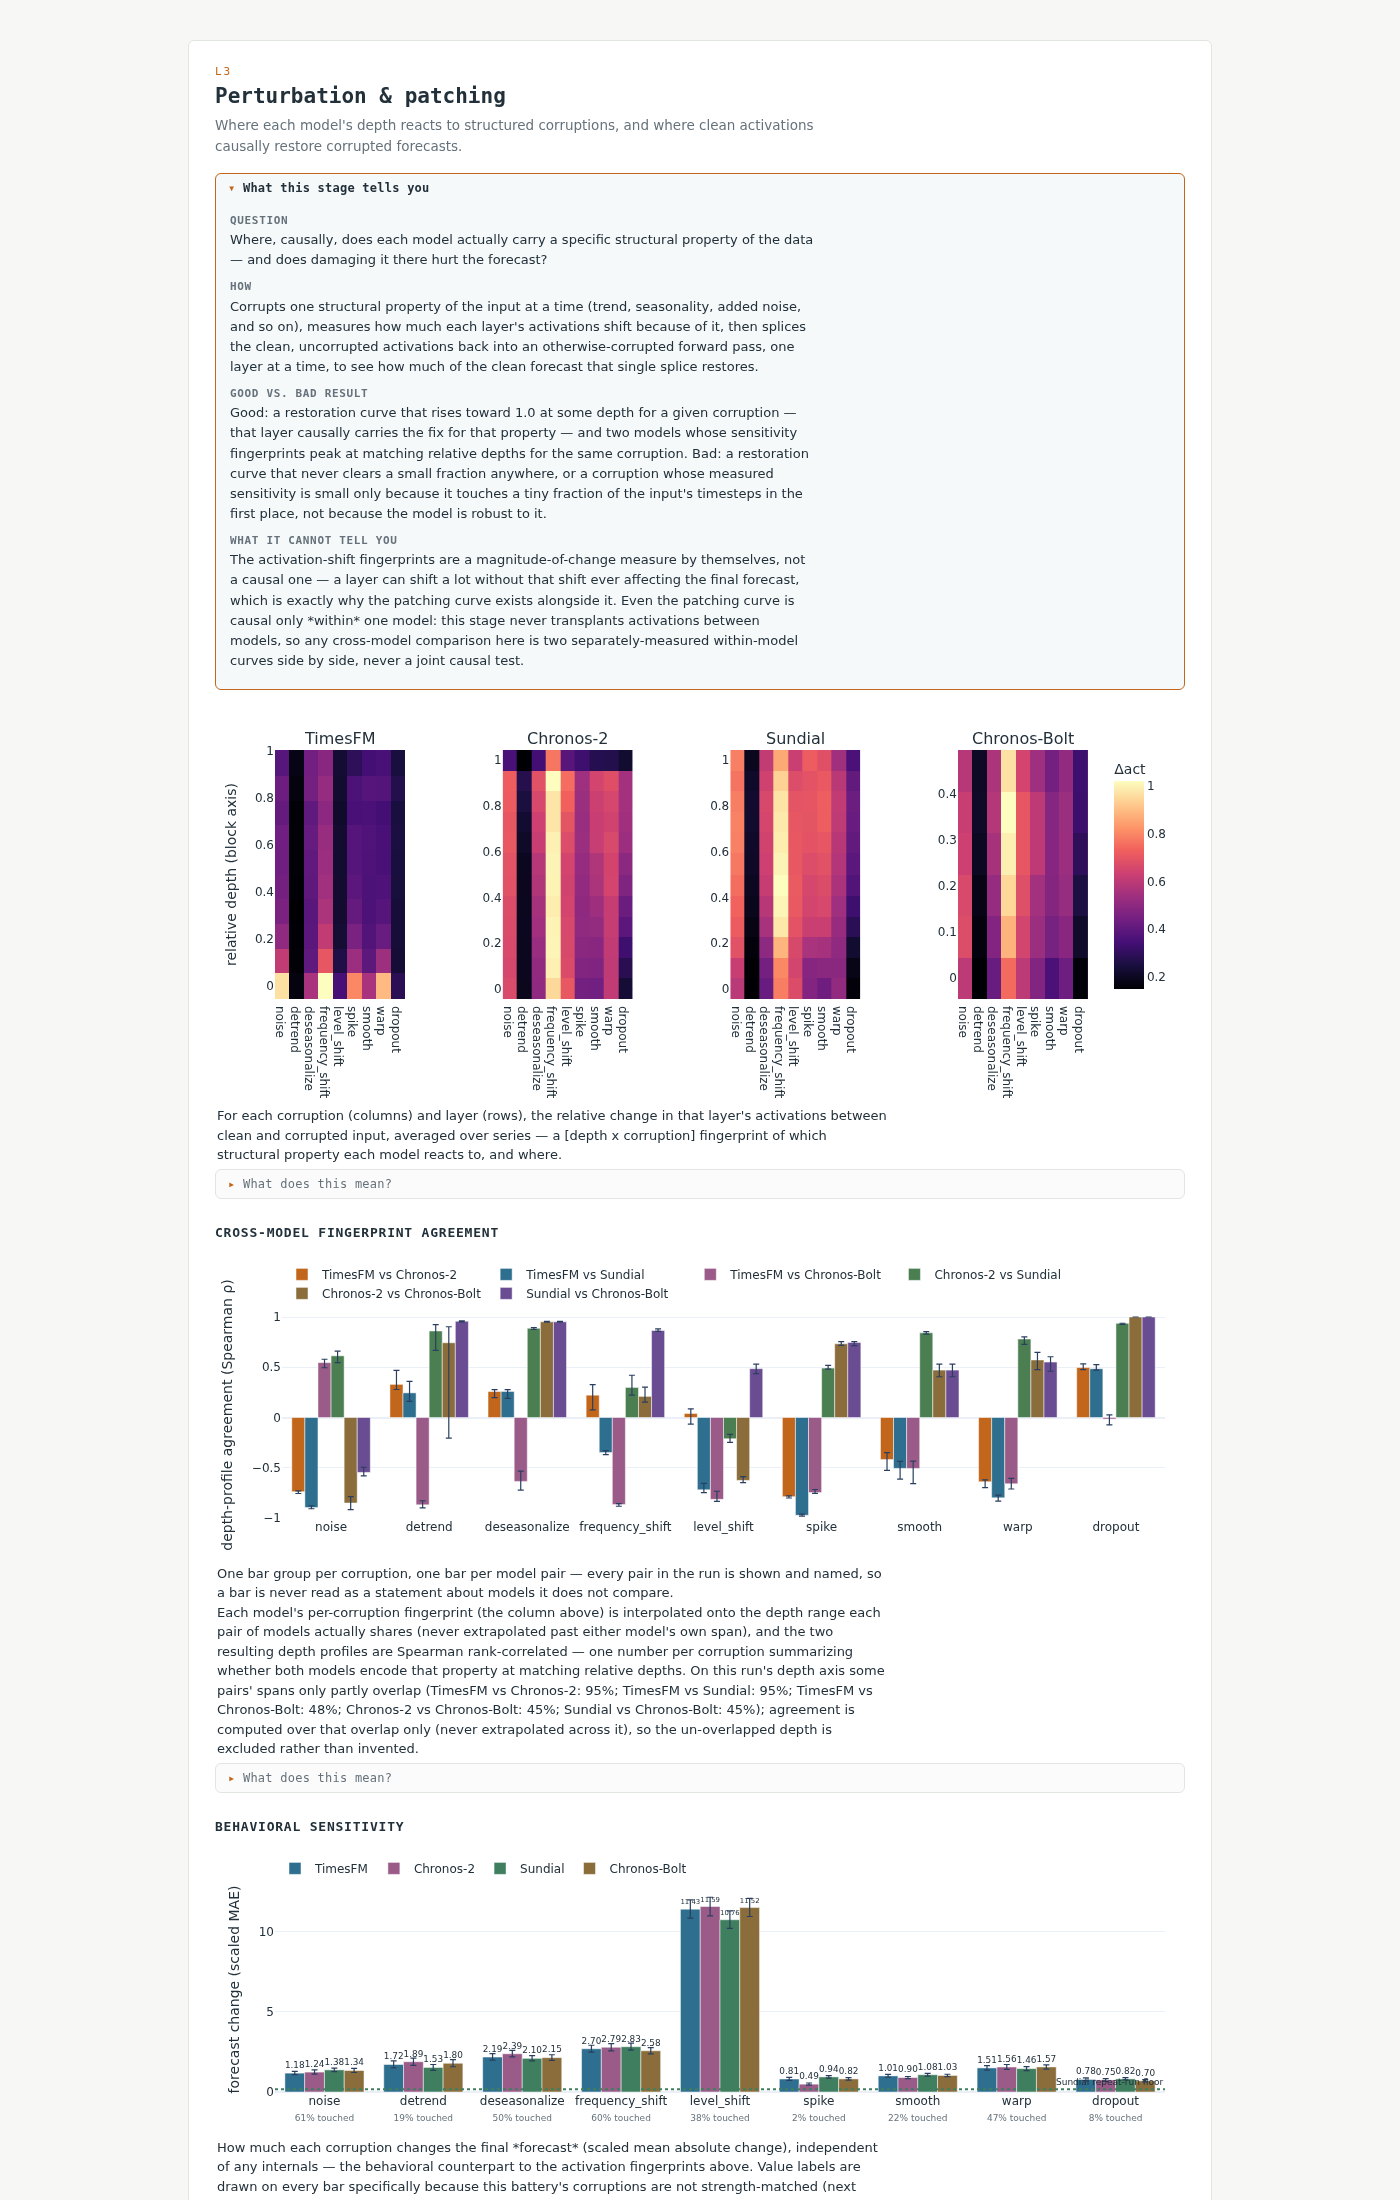
\includegraphics[width=0.86\textwidth]{figures/report_sec-l3.png}
\caption{A stage section (L3, perturbation and patching). The open card states the question, the method,
what a good and a bad result look like and what the analysis cannot tell you; each figure has a caption and a
collapsible ``What does this mean?'' note.}
\label{fig:report-l3}
\end{figure}

\begin{figure}[p]
\centering
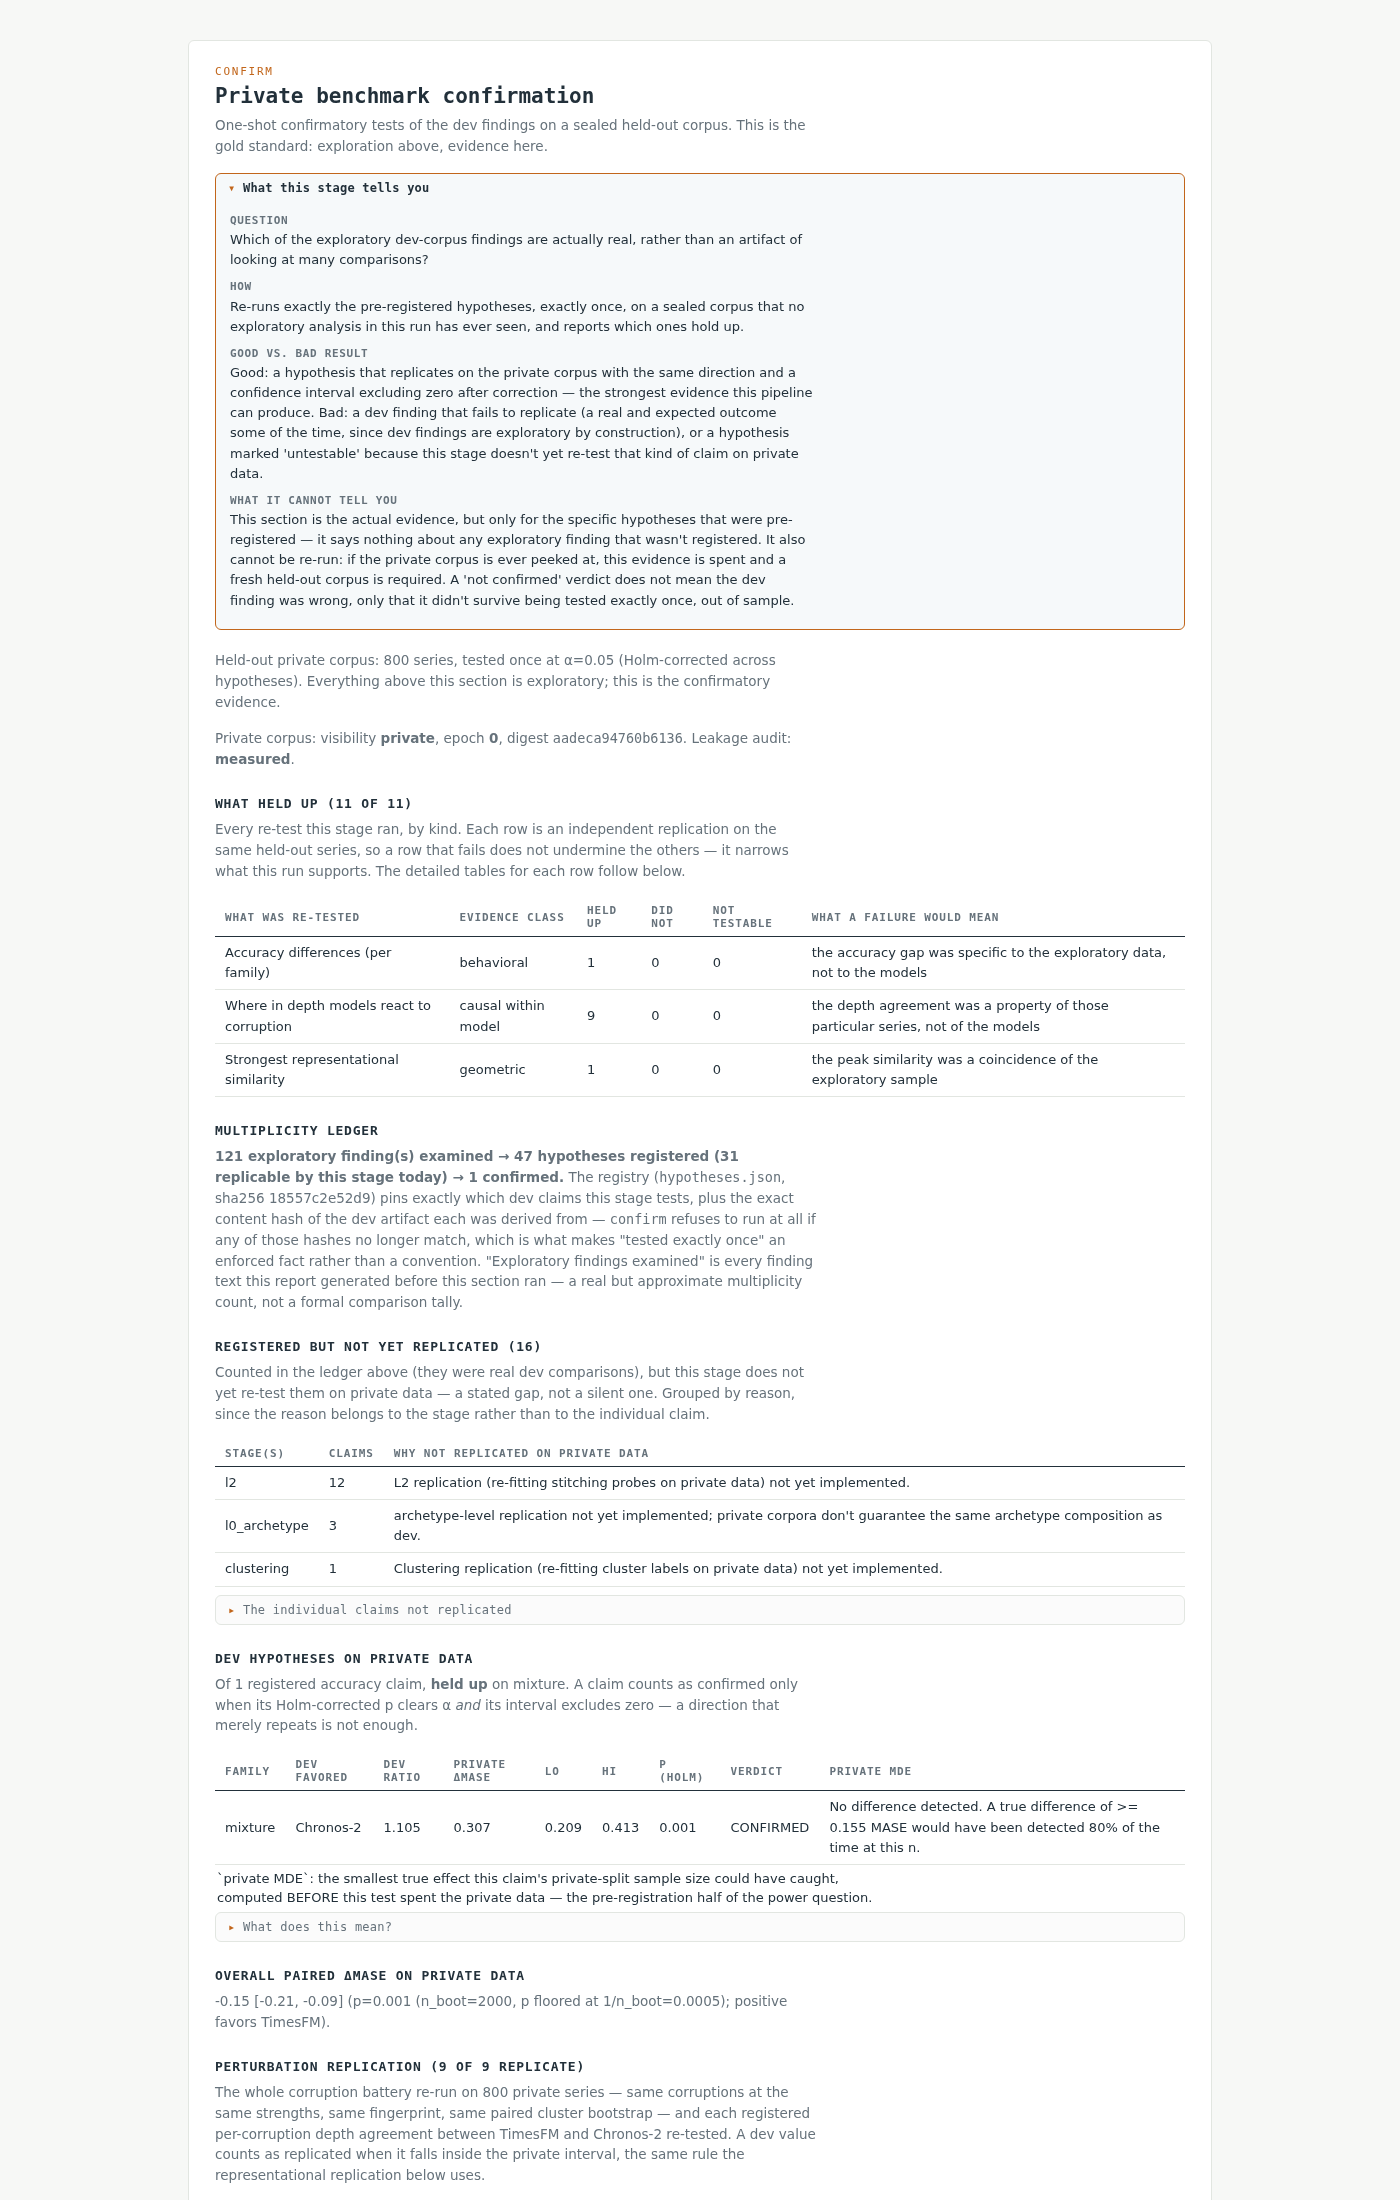
\includegraphics[width=0.86\textwidth]{figures/report_sec-confirm.png}
\caption{The confirmation section: what held up, the multiplicity ledger from exploratory findings to
registered and confirmed claims, registered claims not yet replicable with their reasons, and each
registered claim with its private estimate and pre-computed minimum detectable effect.}
\label{fig:report-confirm}
\end{figure}

\section{Adapter Pitfalls: a Worked Case}
\label{app:adapters}

The adapters guide (\repo{tsfm_lens/docs/ADDING_A_MODEL.md}) documents every pitfall we met. The most
instructive is the Sundial normalization bug (\fid{PM-15}), because the pipeline measured it correctly and
it was still misread.

\paragraph{What happened.} Many Hugging Face checkpoints normalize inputs only inside their own
\texttt{generate()} path. Sundial z-scores each series in \texttt{generate()}, but its \texttt{forward()}
defaults to no normalization. \texttt{generate()} was broken on the installed transformers version, so the
adapter called \texttt{forward()} directly and fed the model raw-scale input. The remote code's own
normalizing branch of \texttt{forward()} fails when more than one sample is drawn.

\paragraph{Symptoms.} The \texttt{frontend} stage reported a scale-equivariance residual of 38.43 context
standard deviations at scale 0.001 (the other models: at most 0.009), and forecasts on large-valued
electricity series were 100\% flat (MASE 4.134, against 24--32\% flat for the other models). The residual was
first recorded as a property of the model.

\paragraph{Fix and lesson.} The adapter now normalizes in \texttt{prepare()} with the checkpoint's exact rule
(standard deviation plus $10^{-5}$) and denormalizes samples in \texttt{predict()}, in one place, so capture,
prediction and patching see identical inputs. The residual fell to 0.030 and the flat share on electricity to
0.08; the same defect in the zero-code adapter on Timer fell from 49.73 to 0.020. The report now flags any model
whose residual exceeds $\max(1, 10\times$ the peers' median$)$. The lesson generalizes: an adapter that calls a
model below its public API must reproduce everything that API does to the input and output.

\paragraph{Checklist.} The guide's checklist, each item with a reason and a check: input normalization
(frontend residual); seeded sampling for sampled heads, with identical seeds in every compared pair of calls
(two unpatched predictions must match); clean-cache precision matching \texttt{predict()}; no silent batch
chunking during patching; anchored layer regular expressions; contiguous token spans (measured by span
discovery, verified by the alignment gate); routing of non-time-localized models; stating which part of an
encoder--decoder is captured; reach controls (self-patch exactly 0, cross-patch nonzero); random-weight twins
checked for reach before use as a causal floor; original-scale outputs; rerunning
\texttt{-{}-discover-layers}, \texttt{-{}-check-alignment} and \texttt{-{}-check-adapter} after any library or
checkpoint change; and adapter tests with a planted answer and a decoy.
